\documentclass{article}
\usepackage{pgfplots}
\begin{document}
\section{Creating Plots and Graphs}

The \texttt{pgfplots} package in LaTeX allows for powerful plotting capabilities. Below are some examples of how to create simple 2D and 3D plots.

\subsection{Example of a 2D plot}
\begin{center}
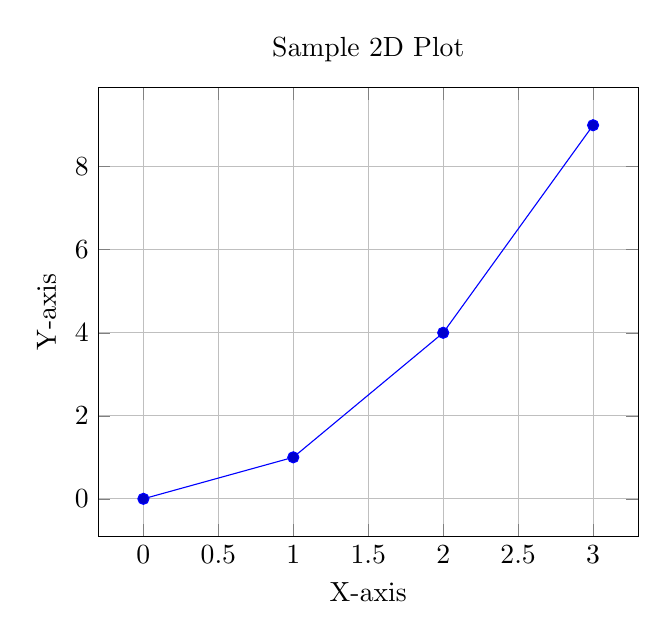
\begin{tikzpicture}
\begin{axis}[
    title={Sample 2D Plot},
    xlabel={X-axis},
    ylabel={Y-axis},
    grid=both
]
    \addplot coordinates {(0,0) (1,1) (2,4) (3,9)};
\end{axis}
\end{tikzpicture}
\end{center}

\subsection{Example of a 3D plot}
\begin{center}
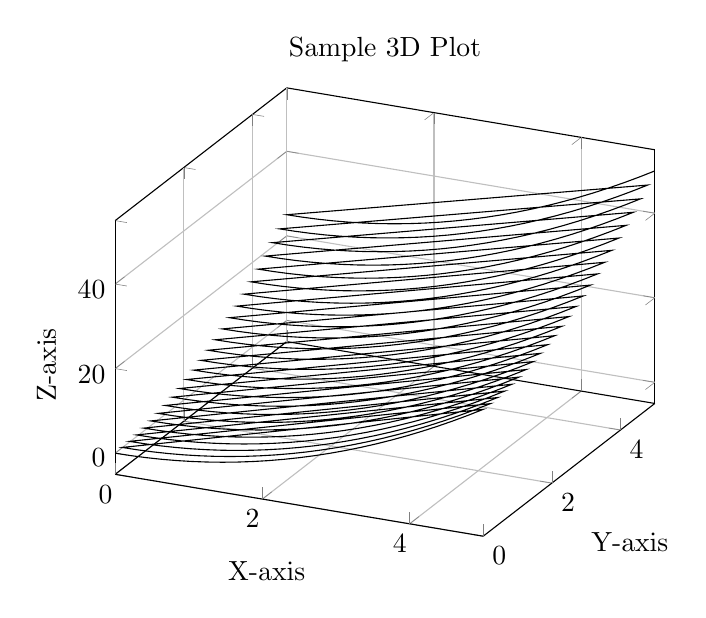
\begin{tikzpicture}
\begin{axis}[
    title={Sample 3D Plot},
    xlabel={X-axis},
    ylabel={Y-axis},
    zlabel={Z-axis},
    grid=major
]
    \addplot3[domain=0:5] {x^2 + y^2};
\end{axis}
\end{tikzpicture}
\end{center}

\end{document}